
\documentclass[journal]{IEEEtran}
\usepackage{blindtext}
\usepackage{graphicx}


\ifCLASSINFOpdf
  % \usepackage[pdftex]{graphicx}
  % declare the path(s) where your graphic files are
  % \graphicspath{{../pdf/}{../jpeg/}}
  % and their extensions so you won't have to specify these with
  % every instance of \includegraphics
  % \DeclareGraphicsExtensions{.pdf,.jpeg,.png}
\else
  % or other class option (dvipsone, dvipdf, if not using dvips). graphicx
  % will default to the driver specified in the system graphics.cfg if no
  % driver is specified.
  % \usepackage[dvips]{graphicx}
  % declare the path(s) where your graphic files are
  % \graphicspath{{../eps/}}
  % and their extensions so you won't have to specify these with
  % every instance of \includegraphics
  % \DeclareGraphicsExtensions{.eps}
\fi

% correct bad hyphenation here
\hyphenation{op-tical net-works semi-conduc-tor}
\usepackage{amsmath, amsthm, amssymb, amsfonts}

\begin{document}

%
% paper title
% can use linebreaks \\ within to get better formatting as desired
\title{Group 80: Pattern Classification and Machine Learning Project1}


\author{Alper~Kose,
        Romain~Choukroun,
        and~Hugo~Bonnome
}


\maketitle


\begin{abstract}

The aim of this paper is to classify Higgs Boson experiment's results using six machine learning methods. We will lay out our full thought process, from feature engineering to the evaluation of all methods. Finally, we will explain why the regularized Logistic Regression will fit best our data.



\end{abstract}
% IEEEtran.cls defaults to using nonbold math in the Abstract.
% This preserves the distinction between vectors and scalars. However,
% if the journal you are submitting to favors bold math in the abstract,
% then you can use LaTeX's standard command \boldmath at the very start
% of the abstract to achieve this. Many IEEE journals frown on math
% in the abstract anyway.

% Note that keywords are not normally used for peerreview papers.
\begin{IEEEkeywords}
Feature selection, Gradient Descent, Ridge Regression, Logistic Regression, Regularized Regression
\end{IEEEkeywords}


% For peer review papers, you can put extra information on the cover
% page as needed:
% \ifCLASSOPTIONpeerreview
% \begin{center} \bfseries EDICS Category: 3-BBND \end{center}
% \fi
%
% For peerreview papers, this IEEEtran command inserts a page break and
% creates the second title. It will be ignored for other modes.
\IEEEpeerreviewmaketitle



\section{Data Handling and Feature Selection}
The data set consists of 250.000 samples of each 30 features, each of which corresponds to an experiment measurement result. What we are studying here is how to handle the data to a form which would lead to the highest classification accuracy using a machine learning model. To begin with, some measurements had a value of -999, being obvious defects. To solve this issue, we tried a few approaches: for instance, we thought of removing all such defected samples from the data. Quickly, we understood that it would be wrong since we also had these values in our testing set. Next, we noticed that all these defects of measurements reside in 11 specific features. As a result, we removed these dimensions from the training and test sets. At first look, this seemed to be a good solution despite ignoring some meaningful measurements, but when we tested this hypothesis we had a decrease in the accuracy of our classifications. After brainstorming, we finally decided to set them to 0, normalize the data and construct the polynomial basis. \\Things got interesting when constructing the polynomial basis, in fact, we had a trade-off. Constructing more and more features was increasing our classification accuracy but was also leading to higher memory usage and computational burden. To optimize as much as we could this trade-off, we constructed a data set which has 1400 dimensions using the 30 original features. Here is our construction: the first 30 dimensions consist of the original data set, then we constructed the 2$^{nd}$ degree set by combining each feature with one another. After that, we appended simple polynomial basis created all from the original set, from the 3$^{rd}$ degree to the 10$^{th}$ one. Finally, we added the 3$^{rd}$ degree combinations of the first 15 features of the original data set (adding the most correlated dimensions with class labels did not improve our result, so we added the first 15 ones). Our final data set is composed of 250.000 samples and 1400 features without counting the one consisting of only ones.

\section{Methods}

On our path to finding the best model, we tried 6 methods: Linear Regression using Gradient Descent and/or Stochastic Gradient Descent, Least Squares Regression, Ridge Regression using normal equations and finally normal and regularized Logistic Regressions. Since we had a pretty big data set, it seemed obvious to use a validation set to find the best parameters. After finding the best method, we used a 5-fold cross-validation to have more precise results. This allowed us to use 80\% of the data for training and 20\% for testing. Let's see how we actually found this best method.\\
To begin with, using a batch size of 1 (imposed) in Stochastic Gradient Descent, did not give us any satisfying result: for 50 iterations, \textit{gamma}=0.001 lead to a validation accuracy of 0.66538, \textit{gamma}=0.0001 to 0.68028, and \textit{gamma}=0.00001 to 0.67668. Since the batch size was immovable, we knew that increasing the number of iterations or narrowing the grid search would not improve our results much. So we moved on to another method: Gradient Descent, which lead us to good results. Again, using grid search and 500 iterations, \textit{gamma}=0.01 gave a validation accuracy of 0.80956, \textit{gamma}=0.015 of 0.81212 and \textit{gamma}=0.016 of 0.81266, for higher gammas, the accuracy decreased rapidly.
Reflecting on these results, we decided to stop putting in more efforts in order to improve with these two models, since we know that the Least Squares method using normal equations was going to give a better result anyway. This comes right from the fact that it directly implements the optimal solution that Gradient Descent tries to find using iterations. And, as we expected, we got a solid validation accuracy of 0.82528 using on the validation set using Least Squares.
Onto Ridge Regression now, Ridge Regression is like Least Squares but shrinks the estimated coefficients towards zero. Namely, it has a regularization parameter \textit{lambda} used to avoid  overfitting. Considering our polynomial basis, it was likely that some overfitting was going to take place during the training. While implementing the Ridge Regression, we tuned the \textit{lambda} using some validation, but since Ridge Regression was probably going to compete with the Logistic one for the trophy, we focused more on the calculation of \textit{lambda} by using a 5-fold cross-validation. And finally, we obtained a higher accuracy than the Least Squares method. Here are the average cross-validation accuracies according to different \textit{lambda} values:  \textit{lambda}=10\textsuperscript{-12} gave us 0.82875, \textit{lambda}=10\textsuperscript{-13} showed  0.82931 and \textit{lambda}=10\textsuperscript{-14}, 0.82922. Nearly 83\% classification accuracy was observed with a very small regularization parameter which proved that there was not really any significant overfitting.
Finally, it was time to implement the Logistic and Regularized Logistic Regressions. For the methods that we discussed until now, we have used standard formulas that we saw in class. As for the Logistic Regressions, we used the Newton Method since we benefit from the second degree calculation and provides a greater and quicker convergence. We came up with a somewhat different formula for the gradient:

\begin{equation}
\mathbf{grad(w)}=-\dfrac{1}{N}\sum_{n=1}^{N} \dfrac{y_{n}\mathbf{x_{n}}}{1+\exp(y_{n}\mathbf{w^{T}}\mathbf{x_{n}})}
\end{equation}
where N is the number of data points used in the training. We then computed pretty much the same Hessian that we saw in class:

\begin{equation}
\mathbf{H(w)=X^{T}SX} 
\end{equation}
\begin{equation}
\mathbf{S}=\sigma(\mathbf{x_{n}w})[1-\sigma(\mathbf{x_{n}w})]
\end{equation}
\begin{equation}
\mathbf{w}=\mathbf{w}-gamma*\mathbf{grad(w)}*\mathbf{H^{-1}(w)}
\end{equation}
where  $\sigma$ is the sigmoid function. By implementing the Logistic Regression, we reached an even higher classification accuracy. This was to be expected, since the Logistic Regression is one of the most widely used and successful technique in classification compared to the others we tried beforehand. During our regression, we multiplied \textit{gamma} with 0.55 every 5 iterations to be able to begin with a higher value and have a refined convergence. In the grid search, we encountered several singular value errors with some values of \textit{gamma}, which was normal since we changed all the defected -999s values to 0 in the data set. On the other hand, \textit{gamma} values that did not result in such singular value errors gave us very good results, namely higher classification accuracies than the Ridge Regression. In terms of experimental results, we reached 0.83655 on average validation accuracy when \textit{gamma}=80000, 0.83399 when \textit{gamma}=80050 and 0.83631 when \textit{gamma}=79600. So we obtained a high classification accuracy with the Logistic Regression, as expected. On the other hand, since ill-posed matrix ruined the training process of many \textit{gamma} values, we thought that a regularization could give even better results by coping with the ill-posed nature of the problem.


\section{Regularized Logistic Regression (WINNER)}

Finally, we moved onto Regularized Logistic Regression to complete the project. We also used the equations (1) and (3) as we did before, whereas the equations (2) and (4) underwent minor changes:

\begin{equation}
\mathbf{H(w)=X^{T}SX+I} 
\end{equation}
\begin{equation}
\mathbf{w}=\mathbf{w}-gamma*\mathbf{grad(w)}*\mathbf{H^{-1}(w)}-gamma*lambda*\mathbf{w}
\end{equation}

where \textbf{I} is the identity matrix and lambda the regularization parameter. The final running time was approximately half an hour with 25 iterations and 5-folds cross-validation. Therefore, we could not have searched an extensive grid for parameters \textit{lambda} and \textit{gamma}. To overcome this difficulty, we started by searching in a large grid using one validation set and trying parameter values which we input by hand in every trial. After estimating the value intervals that lead to high accuracy, we did a small grid search where the possible values were \textit{lambda}=[5*10\textsuperscript{-9},10\textsuperscript{-8},2*10\textsuperscript{-8}] and \textit{gamma}=[8*10\textsuperscript{4}, 9*10\textsuperscript{4}, 10*10\textsuperscript{4},11*10\textsuperscript{4}, 12*10\textsuperscript{4}]. And after doing a 5-folds cross-validation, the classification accuracy came to be as in Figure1.

\begin{figure}[h]
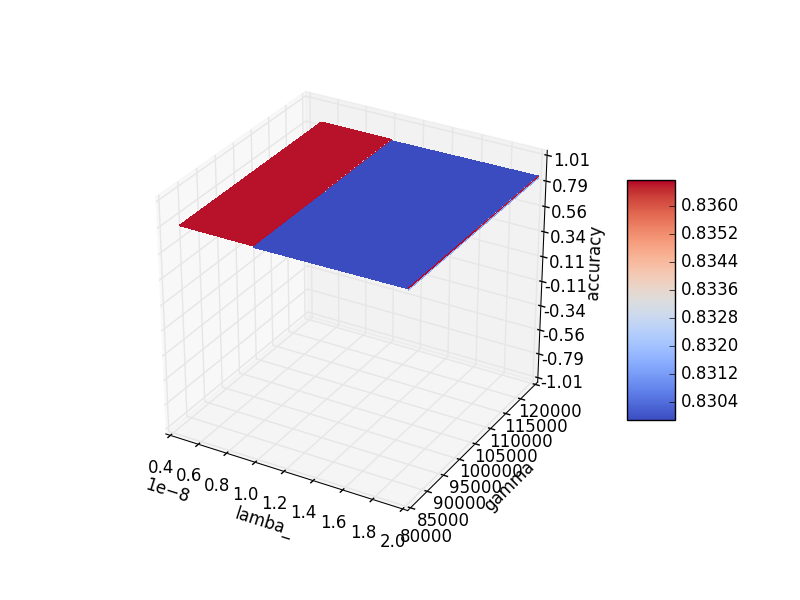
\includegraphics[width=0.4\textwidth]{figure_1.png}
\caption{Average validation accuracy results for 5-folds cross-validation}
\end{figure}



Even from the figure, it was hard to choose the best pair of values since the accuracies were so close. Still, the (\textit{lambda}=10\textsuperscript{-8}  , \textit{gamma}=10\textsuperscript{5}) pair gave the highest average validation accuracy which was 0.83674. In order to get an even better accuracy, the 5 different weights, the results of the 5-folds cross-validation, were averaged. As desired, this further increased the classification accuracy by 0.001 in the test set.


\section{Conclusion}

Submitting our final solution to Kaggle, we achieved a 0.83782 score which seemed pretty high when compared to other groups. Although our results are good, there is still room for improvement. On the last day of submission, we realized that the 23$^{rd}$ feature of the original data set was consisting only of categorical values 0, 1, 2 and 3. So if the data were to be divided into four subsets, four different weight vectors could be trained separately and the labels of the tests set could be found by dividing the test set in four, according to categorical value of the samples and the related weight vectors used to estimate the labels. Also, wider grid search can be used to estimate the parameters of the functions. But since there is a trade-off between classification accuracy and computation time, when we add more and more degrees of polynomial basis, this makes grid search way harder to compute but increases the accuracy when suitable parameters are found. Finally, as a suggestion for next years project, if supercomputers(clusters) in labs could be made available to students, so that they can test their algorithm without losing too much time and achieve better and more interesting results.






\ifCLASSOPTIONcaptionsoff
  \newpage
\fi



\begin{thebibliography}{1}

\bibitem{IEEEhowto:kopka}
https://work.caltech.edu/library/093.pdf

\bibitem{IEEEhowto:kopka}
http://mlo.epfl.ch/page-136795.html


\end{thebibliography}




\end{document}


